\documentclass[11pt,letterpaper]{article}
\usepackage[utf8]{inputenc}

%----- Configuración del estilo del documento------%
\usepackage{epsfig,graphicx}
\usepackage[left=2cm,right=2cm,top=1.8cm,bottom=2.3cm]{geometry}
\usepackage{fancyhdr}
\usepackage{lastpage}
\usepackage{url}
\pagestyle{fancy}
\fancyhf{}
\rfoot{\textit{Página \thepage \hspace{1pt} de \pageref{LastPage}}}


%------ Paquetes matemáticos básicos --------%
\usepackage{amsmath}
\usepackage{amssymb}
\usepackage{amsthm}

\usepackage[spanish]{babel}
\usepackage{graphicx}
\usepackage{hyperref}

\usepackage{tabularx}
\usepackage{xcolor}
\usepackage[table]{xcolor}
\usepackage{colortbl}
\usepackage{array, multirow, multicol, tabularx}
\usepackage{tcolorbox}
\newtheorem{theorem}{Theorem}[section]
\newtheorem{corollary}{Corollary}[theorem]
\newtheorem{lemma}[theorem]{Lemma}

%------si-------%
\definecolor{B}{HTML}{FFFFFF}
\definecolor{G}{HTML}{5e5e5e}
\definecolor{R2}{HTML}{d53d40}
\definecolor{A2}{HTML}{034190}
\definecolor{V2}{HTML}{7faa50}
\newcommand{\R}{\mathbb{R}}
\newcommand{\C}{\mathcal{C}}
\newcommand{\Z}{\mathbb{Z}}
\newcommand{\Q}{\mathbb{Q}}
\newcommand{\N}{\mathbb{N}}
\newcommand{\Li}{\mathfrak{L}}
\renewcommand{\theenumi}{\Roman{enumi}}
\renewcommand{\labelenumi}{{\theenumi}.}

\begin{document}
\makeatletter
        \renewenvironment{proof}[1][\proofname]{\par
            \pushQED{\qed}%
            \normalfont \topsep6\p@\@plus6\p@\relax
            \trivlist
            \item\relax
            {\itshape
            #1\@addpunct{.}}\par\vspace{\baselineskip}\ignorespaces
            }{%
            \popQED\endtrivlist\@endpefalse
            }
\makeatother
%------ Encabezado -------- %

\begin{center}
    \begin{minipage}{3cm}
    	\begin{center}
    		\includegraphics[height=3.4cm]{logo_unam.png}
    	\end{center}
    \end{minipage}\hfill
    \begin{minipage}{10cm}
    	\begin{center}
    	\textbf{\large Universidad Nacional Autónoma de México}\\[0.1cm]
        \textbf{Facultad de Ciencias}\\[0.1cm]
        \textbf{\'Algebra lineal}\\[0.1cm]
        Tarea examen 1 \\[0.1cm]
         El\'ias L\'opez Rivera$^{1}$\,\,Adolfo Angel Cardoso Vasquez$^{2}$\\[0.1cm]
        Fecha:\,\,12/07/2025
    	\end{center}
    \end{minipage}\hfill
    \begin{minipage}{3cm}
    	\begin{center}
    		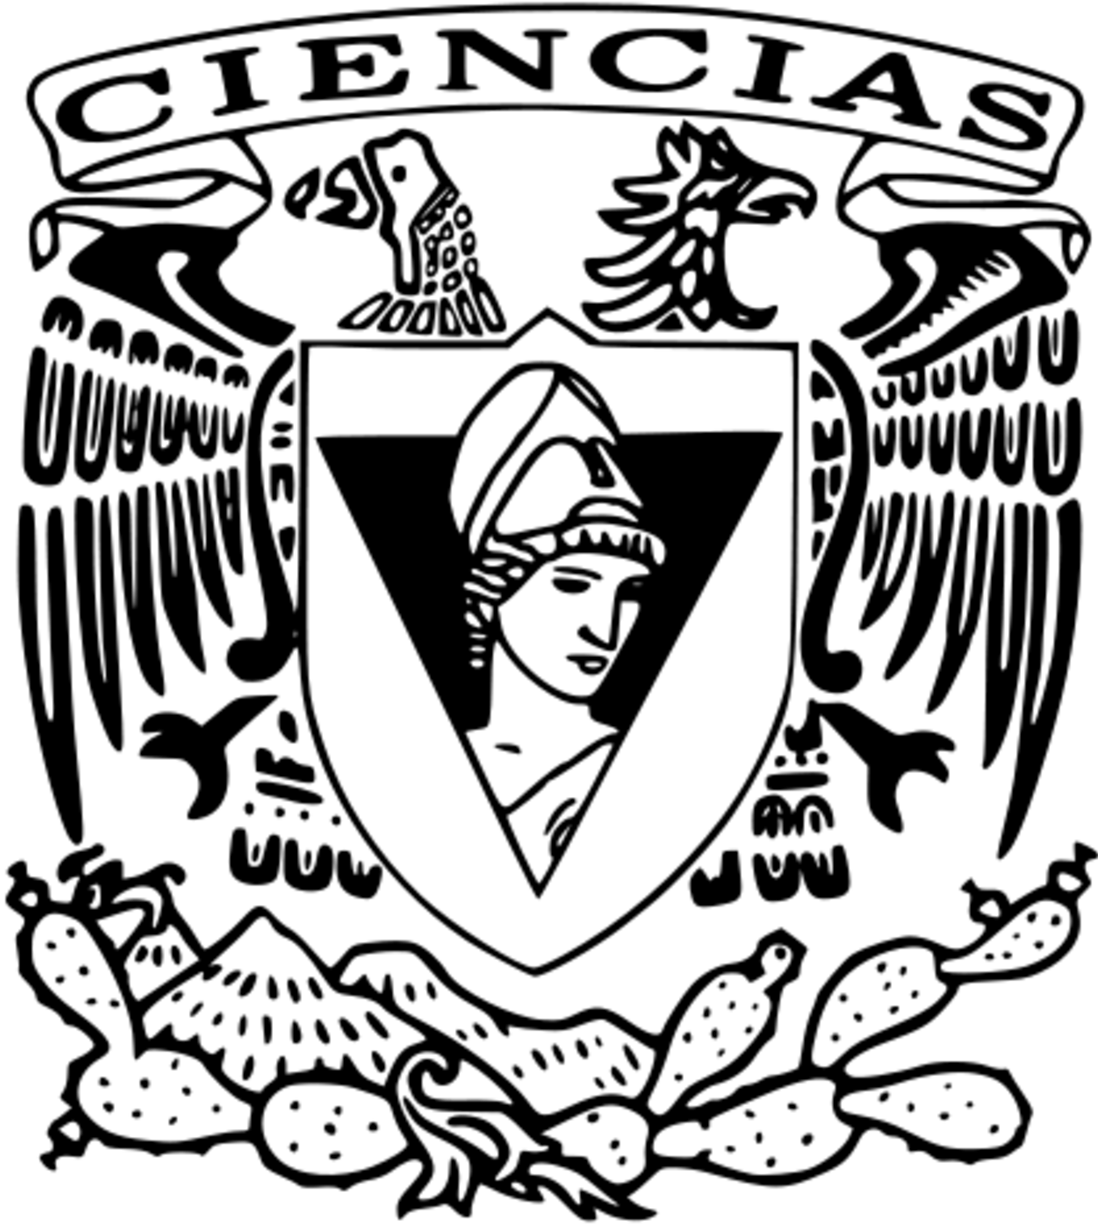
\includegraphics[height=3.4cm]{Logo_FC.png}
    	\end{center}
    \end{minipage}
\end{center}

\rule{17cm}{0.1mm}

%------ Fin de encabezado -------- %
\begin{tcolorbox}[title=Problema 1, colframe=G, coltitle=B, fonttitle=\bfseries]
\textit{Demostrar que para cualquier tri\'angulo $\Delta\,ABC$ se cumple que $\sin(A)\,\sin(B)\,\sin(C)\leq\frac{3\sqrt{3}}{8}$, ademas se tiene la igualdad si y solo si el tri\'angulo es
equilatero}  
\end{tcolorbox}
\begin{proof}\,\\
    \,\\
\end{proof}
\begin{tcolorbox}[title=Problema 2, colframe=G, coltitle=B, fonttitle=\bfseries]
\textit{Calcular la siguiente integral:
\begin{equation*}
    \int_{0}^{1}\,\frac{x^{cos(x)}-1}{ln(x)}
\end{equation*}}  
\end{tcolorbox}
\begin{proof}\,\\
    \,\\
\end{proof}
\begin{tcolorbox}[title=Problema 3, colframe=G, coltitle=B, fonttitle=\bfseries]
\textit{Expresar el siguiente polinomio como cociente (no trivial) de dos polinomios:
\begin{equation*}
  \frac{f(x)}{g(x)}=2x+4x^3+\cdots+(2n)x^{2n-1}
\end{equation*}}  
\end{tcolorbox}
\begin{proof}\,\\
    \,\\
\end{proof}
\begin{tcolorbox}[title=Problema 4, colframe=G, coltitle=B, fonttitle=\bfseries]
\textit{Si $\theta=\alpha,\beta$ son raices de la ecuaci\'on $a\cos(\theta)+b\sin(\theta)=c$, demuestra que:
\begin{equation*}
  \cos(\alpha+\beta)=\frac{a^2-b^2}{a^2+b^2}
\end{equation*}}  
\end{tcolorbox}
\begin{proof}\,\\
    \,\\
\end{proof}
\begin{tcolorbox}[title=Problema 5, colframe=G, coltitle=B, fonttitle=\bfseries]
\textit{Hallar $X\in M_{3}(\R)$ tal que:
\begin{equation*}
  AXA^{T}=\begin{pmatrix}
    0 & 0 & 0 & 0\\
    0 & 2017 & 7(2017) & 2(2017)\\
    0 & 7(2017) & 49(2017) & 14(2017)\\
    0 & 2(2017) & 14(2017) & 4(2017)\\
  \end{pmatrix}\,\,\,\,con\,\,\,\,A=\begin{pmatrix}
    2 & 0 & 2\\
    0 & 1 & 0 \\
    1 & 7 & 1 \\
    7 & 2 & 7\\
\end{pmatrix}
\end{equation*}}  
\end{tcolorbox}
\begin{proof}\,\\
    \,\\
\end{proof}
\end{document}